\section{Model-View-Controller}
\label{sec:mvc}

To Model-View-Controller (εν συντομία \textbf{MVC}) είναι ένα σχεδιαστικό πρότυπο ευρέως διαδεδομένο, ειδικά στην ανάπτυξη Web εφαρμογών και απεικονίζεται στο Σχήμα \ref{fig:mvc}. Όπως προδίδει και το όνομά του, το MVC χρησιμοποιεί 3 είδη κλάσεων οι οποίες περιγράφονται παρακάτω \cite{MVCPaper}.

\begin{figure}[h]
    \centering
    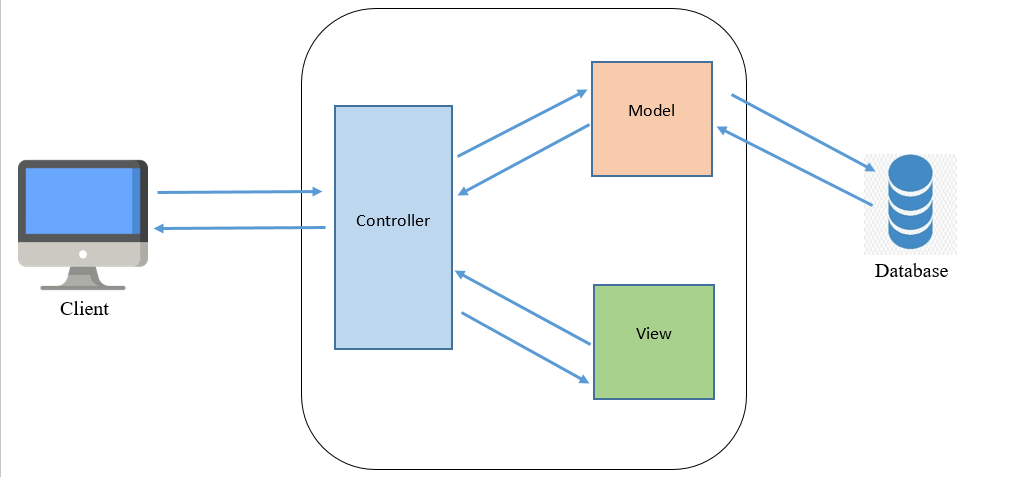
\includegraphics[scale=0.41]{images/chapter4/mvc.png}
    \caption{Αρχιτεκτονική MVC}
    \label{fig:mvc}
\end{figure}

\begin{itemize}
    \item \textbf{Model}: Οι συγκεκριμένες κλάσεις χρησιμοποιούνται για την αλληλεπίδραση με τα δεδομένα, δηλαδή την εισαγωγή, την ανάκτηση και την ενημέρωση των βάσεων δεδομένων της εφαρμογής 
    \item \textbf{View}: Υλοποιούν με γραφικό τρόπο την διεπαφή της εφαρμογής μέσω της οποίας αλληλεπιδρούν οι χρήστες.
    \item \textbf{Controller}: Ακούνε τα αιτήματα των χρηστών και εκτελούν τις κατάλληλες ενέργειες. Οι κλάσεις αυτές αλληλεπιδρούν με τις Model και επιλέγουν το κατάλληλο View για να εμφανίσουν στον χρήστη ανάλογα με τις ενέργειες που απαιτεί.
\end{itemize}

Βλέπουμε επομένως ότι το MVC είναι ένα πρότυπο 3 επιπέδων το οποίο ορίζει εκτός από τα επίπεδα και τις σχέσεις μεταξύ αυτών (Σχήμα \ref{fig:mvc}). Πιο συγκεκριμένα, το επίπεδο του Controller αλληλεπιδρά με τον χρήστη λαμβάνοντας δεδομένα τα οποία τα αποστέλλει στο Model επίπεδο αφού πρώτα τα επικυρώσει. Επίσης, ανάλογα με το αίτημα του χρήστη θα ζητήσει τα κατάλληλα δεδομένα από το Model προκειμένου να τα αποστείλει στο επίπεδο View για να δημιουργηθεί η κατάλληλη απεικόνιση για τον χρήστη.

Τέλος, το συγκεκριμένο πρότυπο προσφέρει αρκετά πλεονεκτήματα όπως:

\begin{itemize}
    \item Μας βοηθάει να ελέγξουμε την πολυπλοκότητα της εφαρμογής χωρίζοντας την σε 3 επίπεδα.
    \item Επιτρέπει ευκολότερες δοκιμές (testing) της εφαρμογής.
    \item Διαφορετικοί προγραμματιστές μπορούν να δουλεύουν ταυτόχρονα στα διαφορετικά επίπεδα κάτι που μειώνει τον χρόνο ανάπτυξης της εφαρμογής.
    
\end{itemize}